%%%%%%%%%%%%%%%%%%%%%%%%%%%%%%%%%%%%%%%%%
% Journal Article
% LaTeX Template
% Version 1.4 (15/5/16)
%
% This template has been downloaded from:
% http://www.LaTeXTemplates.com
%
% Original author:
% Frits Wenneker (http://www.howtotex.com) with extensive modifications by
% Vel (vel@LaTeXTemplates.com)
%
% License:
% CC BY-NC-SA 3.0 (http://creativecommons.org/licenses/by-nc-sa/3.0/)
%
%%%%%%%%%%%%%%%%%%%%%%%%%%%%%%%%%%%%%%%%%

%----------------------------------------------------------------------------------------
%	PACKAGES AND OTHER DOCUMENT CONFIGURATIONS
%----------------------------------------------------------------------------------------

\documentclass{article}

\usepackage{blindtext} % Package to generate dummy text throughout this template 

\usepackage{tikz}
\usetikzlibrary{arrows.meta}
\usepackage{adjustbox}

% define style for ``not visible nodes and edges''
\tikzset{bled/.style={black!40, line width=1pt, fill=white}}

\usepackage{graphicx}



\usepackage[english]{babel} % Language hyphenation and typographical rules




\usepackage{hyperref} % For hyperlinks in the PDF

\title{Understandable Bayesian Recommendation Engine}
%\author{Martin Molan \\
%	Jozef Stefan International Postgraduate School  \\
%	\and 
%	T \\
%	His Company / University \\
%	}

% Hint: \title{what ever}, \author{who care} and \date{when ever} could stand 
% before or after the \begin{document} command 
% BUT the \maketitle command MUST come AFTER the \begin{document} command! 





\begin{document}

% Print the title
\maketitle

%----------------------------------------------------------------------------------------
%	ARTICLE CONTENTS
%----------------------------------------------------------------------------------------
 

\section{Scalable Bayesian approach}
Scalable Bayesian approach is build on idea presented in True Skill algorithm developed by Microsoft Research \cite{TrueSkill}. Approach was developed to model interaction of players in multiplayer games and to predict outcomes of such games. The basic idea is similar to ELO rating in chess and is based on predicted skill of two opponents and their interactions.  Based on the interaction, the skill estimates (model priors) are updated so that:
\begin{itemize}
\item{Score of the winner is increased and score of the looser is decreased.}
\item{Score update (increase for the winner and decrease for the user) depends on the relative skills of the opponents. If the skill difference is big the updates are big and vice versa.}
\end{itemize}
The problem with this approach is that the learning rate (update size) is determined only by difference in skills. That means that skill estimation for a new player takes a relatively long time and that an accidental bad performance can ruin a player's score. This is the problem True Skill aims to address with modeling player score as a Gaissian random variable instead of as a scalar value. Having additional information about the parameter value (parameter variance) means that updates can also be determined by variance. That means that the magnitude of updates and conversely learning speed depends on the amount of information we have about the player. Learning speed is higher (big updates) for new player and smaller for established players. Addition of variance enables the model to learn quicker in generally requires less iterations to estimate player's skill \cite{TrueSkill}.

\subsection{Generalizations of True Skill}
The basic idea of True Skill can be adopted to other problems where basic interaction can be modeled as opposition between two agents. Example of that is True Learn, developed by Bulathwela and others \cite{Sahan}. True Learn is being developed to model the learning path of students consuming educational materials. Agents in opposition in True Skill are learner and educational material. Parameters estimated by the model are material difficulty and learner's skill.
\bigbreak
Another generalization of True Skill is recommendation system for blind students developed by Molan and others \cite{Molan}. Here the system aims to learn student's accessibility preferences and use those preferences to rank materials in terms of suitability for a specific student.
\bigbreak
The idea of two opposing agents in Bayesian learning task can also be abstracted to use in a classification setting. Such work was first explored in \cite{AddPredictor}. There, the task was to learn the user preferences for different types of adds. The agent describing the ad was only a collection of active one hot encoded features. Because the add side was not updated, the variance of those active features is set to 0 (in actual implementation the variance is very small positive value to avoid numerical errors). Generalization of the approach, presented in \cite{AddPredictor}, can be implemented as a general classification algorithm. 

\subsection{Opposition based classifier}
Even basic (binary) classification task can in some way be interpreted as an opposition of two agents. The developed approach only works for one-hot encoded discrete (nominal) variables. Generalization to continuous variables is a topic on ongoing research. The starting shape of the data, processed for the developed classifier is presented in a table \ref{tab:TrueRaw}.
\begin{table}[h!]
\caption{Data, prepared for Bayesian opposition classifier}
\centering
\begin{tabular}{|l|l|l|l|l|l|l|l|l|}
\hline
f1 & f2 & f3 & f4 & f5 & ... & f(N-1) & fN & Label \\ \hline
0  & 1  & 1  & 0  & 1  & ... & 1      & 0  & 1     \\ \hline
\end{tabular}
\label{tab:TrueRaw}
\end{table}

\bigbreak
The model iterates over rows of the dataset - model is updated after each row. In order to understand an update after a single row one only has to understand how to construct two opposing teams form a single line in a dataset. One team is represented by active (hot) features (features with value 1) and another is a dummy team consisting of zero mean 'zero'  variance Gaussians. Dummy team is the same size as a feature team. Both teams are presented in a table \ref{tab:teams}. Information about the label is interpreted as the \emph{outcome} of the opposition; if the label is 1 the feature team won - otherwise dummy team won.


\begin{table}[h!]
\caption{Representation of two opposing teams. G(0,0) designates a deformed Gaussian distribution. G(f) denotes a learned Gaussian for a feature $f$.}
\centering
\begin{tabular}{lllll}
\hline
\multicolumn{1}{|l|}{G(f2)}  & \multicolumn{1}{l|}{G(f3)}  & \multicolumn{1}{l|}{G(f5)}  & \multicolumn{1}{l|}{...} & \multicolumn{1}{l|}{G(f(N-1))} \\ \hline
                             &                             & vs.                         &                          &                                \\ \hline
\multicolumn{1}{|l|}{G(0,0)} & \multicolumn{1}{l|}{G(0,0)} & \multicolumn{1}{l|}{G(0,0)} & \multicolumn{1}{l|}{...} & \multicolumn{1}{l|}{G(0,0)}    \\ \hline
\end{tabular}
\label{tab:teams}
\end{table}


\bigbreak
The main advantage of using described scalable Bayesian approach as a classifier is its interpretability.  Learned attribute weights (Gaussians for each feature) can be examined and visualized as a plot. Variance holds additional information compared to scalar weight values as it describes certainty about the estimated weight. Learning schema can also be represented as a graphical model (as presented on figure \ref{f:g}).

\begin{figure}[h!]
\centering
\caption{Factor graph of a Opposition Bayesian classifier.}
\label{f:g}
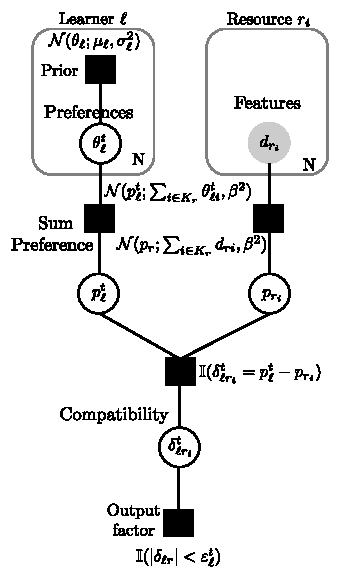
\includegraphics[width=8cm]{fg_true}
\end{figure}


%----------------------------------------------------------------------------------------
%	REFERENCE LIST
%----------------------------------------------------------------------------------------



\begin{thebibliography}{99} % Bibliography - this is intentionally simple in this template
\bibitem{Sahan}
Sahan Bulathwela, M. P.-O.-T. (2020)
\newblock TrueLearn: A Family of Bayesian Algorithms to Match Lifelong Learners to Open Educational Resources
\newblock {\em AAAI Conference on Artificial Intelligence 2020}

\bibitem{TrueSkill}
Herbrich, R. and Minka, T. and Graepel, T. (2007)
\newblock TrueSkill(TM): A Bayesian Skill Rating System
\newblock {\em Advances in Neural Information Processing Systems 20}

\bibitem{Molan}
Molan, M. and Bulathwela, S. and Orlic, D. (2020)
\newblock Accessibility recommendation system
\newblock {\em OER20: Open Education Conference}

\bibitem{AddPredictor}
Graepel, T. and Quiñonero Candela, J. and Borchert, T. and Herbrich, R. (2010)
\newblock Web Scale Bayesian Click Through Rate Prediction for Sponsored Search Advertising in Microsoft’s Bing Search Engine 
\newblock {\em Microsoft Research}

\end{thebibliography}

%----------------------------------------------------------------------------------------

\end{document}
